% Intended LaTeX compiler: pdflatex
\documentclass[11pt]{article}
\usepackage[utf8]{inputenc}
\usepackage[T1]{fontenc}
\usepackage{graphicx}
\usepackage{longtable}
\usepackage{wrapfig}
\usepackage{rotating}
\usepackage[normalem]{ulem}
\usepackage{amsmath}
\usepackage{amssymb}
\usepackage{capt-of}
\usepackage{hyperref}
\author{Fethi Okyar}
\date{2026-03-19}
\title{Chapter 3: The Stress Hypothesis\\\medskip
\large Reading: [Fung/94] Chapter 3}
\hypersetup{
 pdfauthor={Fethi Okyar},
 pdftitle={Chapter 3: The Stress Hypothesis},
 pdfkeywords={},
 pdfsubject={},
 pdfcreator={Emacs 30.2 (Org mode 9.7.11)}, 
 pdflang={English}}
\begin{document}

\maketitle
\setcounter{tocdepth}{1}
\tableofcontents

\section*{(\(\S1.6\)) The Stress/Traction Hypothesis}
\label{sec:org5b7f277}
Consider a material \(B\) occupying a spatial region \(V\). The body is \emph{transmitting} a balanced load system shown with \emph{surface forces} in and \emph{boundary constraints} in . A \textbf{traction field} arises within the body during this transmission. The word \textbf{traction} roughly describes the flow of load per unit area. To \emph{illuminate} the traction field in a region \emph{visualize} an enclosing surface \(S\) around it and \emph{imagine} the interaction between the \emph{inside} (\(-\)) and the \emph{outside} (\(+\)) of \(S\). 
\begin{center}
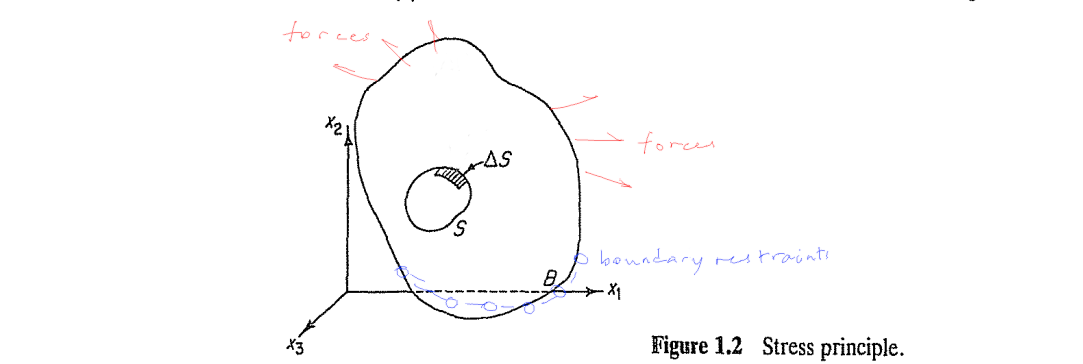
\includegraphics[width=.9\linewidth]{./images/FU94_1.6figure2-load.png}
\end{center}
\subsection*{The Stress/Traction Hypothesis}
\label{sec:orgf739d02}
Let a neighborhood \(\Delta S\) on \(S\) have an \emph{outward unit normal} \(\boldsymbol{\nu}\), with its direction pointing outward from the interior. Let the  \emph{accumulation of load} applied by the (\(+\)) side on the (\(-\)) side passing thru \(\Delta S\) be represented by \(\Delta \mathbf{F}\). The \textbf{stress hypothesis} can be stated: \emph{as} \(\Delta S\) \emph{tends to a small but bounded size} \(\alpha\), \emph{the ratio} \(\Delta \mathbf{F}/\Delta S\) \emph{tends to a definite limit} \(d\mathbf{F}/dS\), \emph{and the moment of the force acting on the surface} \(\Delta S\) \emph{about any point within the area vanishes}. This limiting vector, called as the \textbf{traction} or the \textbf{stress vector} can be written as
$$ \overset{\nu}{\mathbf{T}} = \overset{\nu}{\mathbf{t}} = \frac{d\mathbf{F}}{dS}. $$
\begin{center}
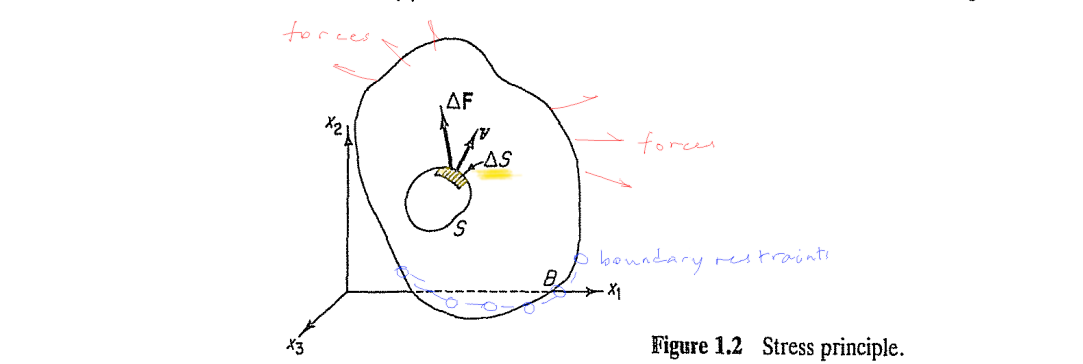
\includegraphics[width=.9\linewidth]{./images/FU94_1.6figure2-deltaS.png}
\end{center}
\subsubsection*{Tractions on Cartesian Planes}
\label{sec:org6dacecf}
\begin{itemize}
\item At an internal point, the standard procedure is to calculate the tractions \(\overset{1}{\boldsymbol{t}}, \overset{2}{\boldsymbol{t}}, \overset{3}{\boldsymbol{t}}\) that arise on the planes cornered by a Cartesian triad \(\boldsymbol{e}_1, \boldsymbol{e}_2, \boldsymbol{e}_3\). 
\begin{center}
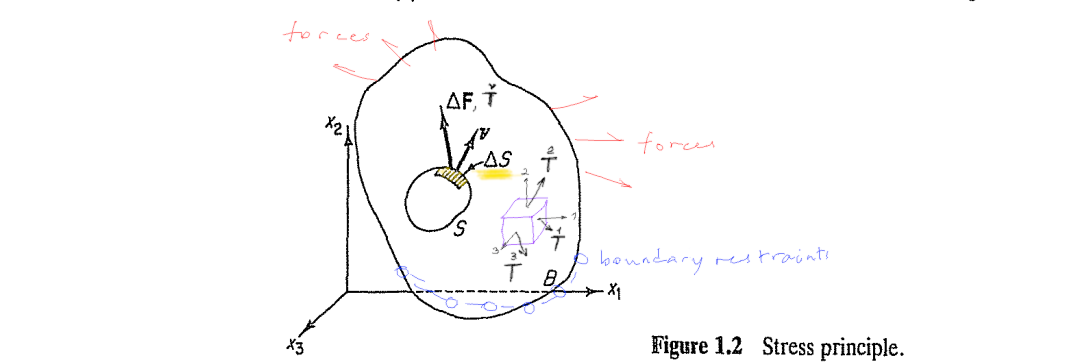
\includegraphics[width=.9\linewidth]{./images/FU94_1.6figure2-tractions.png}
\end{center}
\end{itemize}
\begin{itemize}
\item We combine the three Cartesian tractions as the columns of the transpose of a tensor \(\boldsymbol{\tau}\) as
$$ \left[ \overset{1}{\boldsymbol{t}}, \overset{2}{\boldsymbol{t}}, \overset{3}{\boldsymbol{t}} \right] \triangleq [\tau]^\mathsf{T}  $$
\end{itemize}
\subsubsection*{The Stress Tensor}
\label{sec:org1a7b802}
\begin{itemize}
\item The tensor, \(\boldsymbol{\tau}\), constructed by stacking the three Cartesian internal traction vectors in rows is called as the \textbf{stress tensor}. The stress tensor components read
$$ \begin{bmatrix} \tau_{11} & \tau_{12} & \tau_{13} \\ \tau_{21} & \tau_{22} & \tau_{23} \\ \tau_{31} & \tau_{32} & \tau_{33} \end{bmatrix} = \begin{bmatrix} \overset{ 1}{t_1} & \overset{1}{t_2} & \overset{1}{t_3} \\ \overset{2}{t_1} & \overset{2}{t_2} & \overset{2}{t_3} \\ \overset{3}{t_1} & \overset{3}{t_2} & \overset{3}{t_3} \end{bmatrix} \hspace{2em} \mathrm{or} \hspace{2em} \tau_{ij} = \overset{i}{t_j} $$
\begin{center}
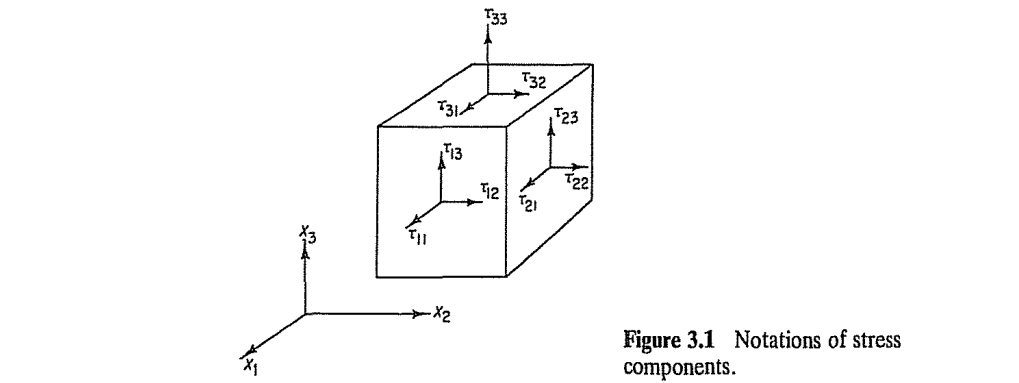
\includegraphics[width=.9\linewidth]{./images/FU94_3.1figure1.png}
\end{center}
\end{itemize}
\subsubsection*{Properties of Internal Traction Vectors}
\label{sec:org704d952}
\begin{itemize}
\item The state of stress at a point in a material is described by internal traction vectors on a differential cube element.
\end{itemize}
\begin{itemize}
\item The differential cube has six faces, three of which have (\(+\)) normals and the other three have (\(-\)) normals.
\item The three traction vectors corresponding to (\(+\)) faces are  \(\overset{1}{\boldsymbol{t}}, \overset{2}{\boldsymbol{t}}, \overset{3}{\boldsymbol{t}}\), and the other three associated with the (\(-\)) faces are \(\overset{-1}{\boldsymbol{t}}, \overset{-2}{\boldsymbol{t}}, \overset{-3}{\boldsymbol{t}}\).
\item The action-reaction principle of Newton can be used to relate the traction vectors on opposite cube faces as
$$ \overset{i}{\boldsymbol{t}} = -\overset{-i}{\boldsymbol{t}} \hspace{2em} \mathrm{or} \hspace{2em} \overset{i}{t_j} = -\overset{-i}{t_j} $$
\item It is standard convention to decompose the traction vector, \(\overset{\nu}{\boldsymbol{t}}\), into it's \textbf{normal} part, \((\boldsymbol{\nu} \cdot \overset{\nu}{\boldsymbol{t}}) \boldsymbol{\nu}\), and it's remaining part, \(\overset{\nu}{\boldsymbol{t}} - (\boldsymbol{\nu} \cdot \overset{\nu}{\boldsymbol{t}}) \boldsymbol{\nu}\), which is \textbf{in-plane} of the surface.
\end{itemize}
\subsubsection*{Properties of Stress Components}
\label{sec:org6245833}
\begin{itemize}
\item In parallel with the parts of the internal traction vectors, the stress components that are normal to the plane are called as \textbf{normal stress} while those components which are in-plane are known as \textbf{shear stress}.
$$ \mathrm{normal} \left\{ \begin{array}{c} \tau_{11} \\ \tau_{22} \\ \tau_{33} \end{array} \right. \hspace{2em} \mathrm{shear}  \left\{ \begin{array}{c} \tau_{12}, \tau_{13} \\ \tau_{21}, \tau_{23} \\ \tau_{31}, \tau_{32} \end{array} \right. $$
\end{itemize}
\begin{itemize}
\item The normal stresses are given a (\(+\)) sign if they point away from the surface (in \textbf{tension}) and a (\(-\)) sign if they point towards the surface (in \textbf{compression}).
\item The shear component (e.g. \(\tau_{ij}\)) is considered as positive if it is acting in the \(+j\) direction on a plane that has a normal in \(+i\) direction, or is in the \(-j\) direction on a plane that has a normal in \(-i\) direction.
\end{itemize}
\subsubsection*{Examples}
\label{sec:org2f7fbe7}
\begin{itemize}
\item Show the following stress components on a differential cube element \(\tau_{11} = 12\) MPa, \(\tau_{21} = -6\) MPa, \(\tau_{31} = 5\) MPa, and \(\tau_{33} = -8\) MPa, with all the remaining stress components identically equan to zero.
\end{itemize}
\begin{itemize}
\item Write the components shown on the stress cube in matrix form.
\begin{center}
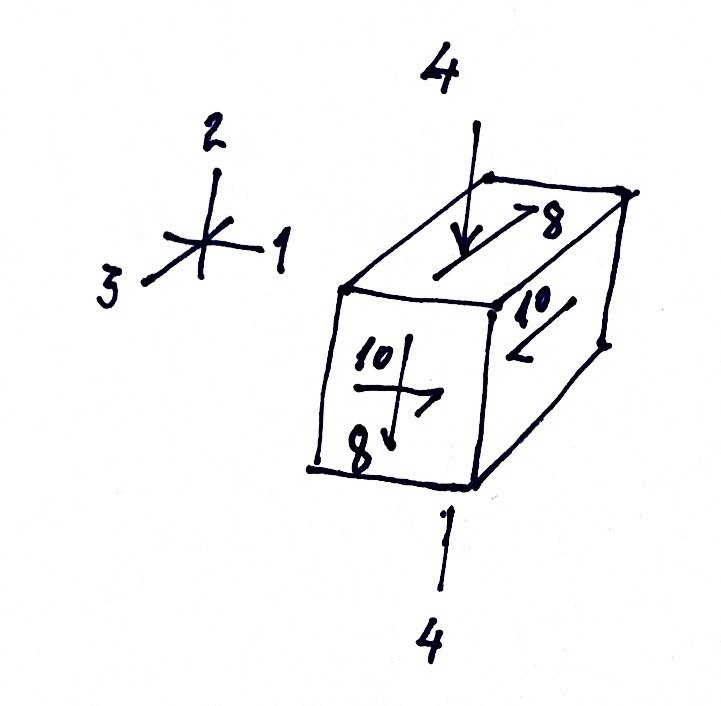
\includegraphics[width=.9\linewidth]{./images/fig3.1-example1.jpg}
\end{center}
\end{itemize}
\section*{(\(\S1.11\)) Examples to Elementary Traction Fields}
\label{sec:org2320c01}
\subsection*{Slender Cylindrical (Axial) Members}
\label{sec:org1e68478}
A \emph{member} (independent part of a structure) is said to be \textbf{\emph{slender}}, if it has a great length to thickness ratio, i.e., \(L/T>>1\), and a constant or slightly-varying cross section swept along the \textbf{normal} to the cross-section plane (a.k.a. member's \emph{longitudinal} or \emph{axial} direction). Such objects in geometry are known as \emph{cylinders}.
\begin{center}
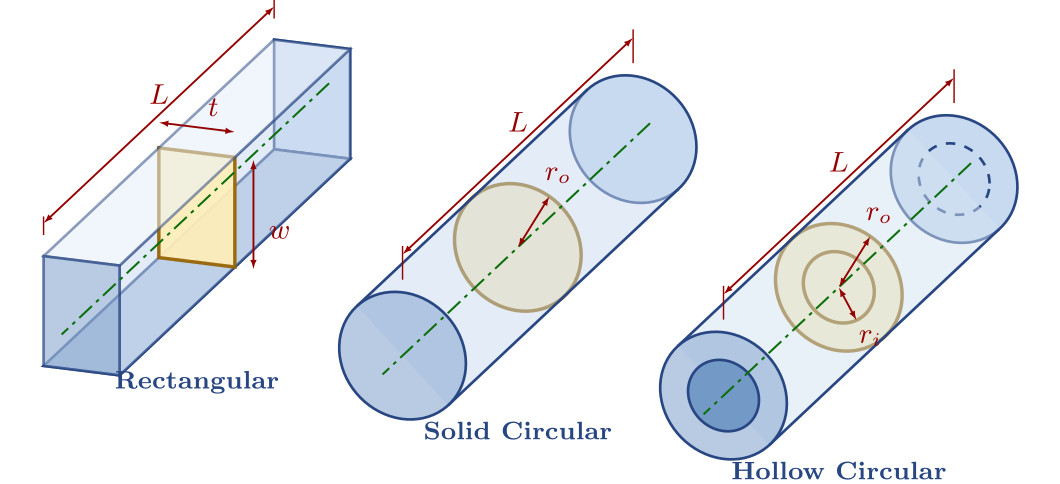
\includegraphics[width=.9\linewidth]{./images/fig1.11.3-members3d.png}
\end{center}
\subsubsection*{Axially Loaded Cylindrical Members}
\label{sec:org0055a70}
\begin{itemize}
\item Consider a member under a \textbf{compressive} force \(W\). We say that the beam is axially loaded without shear. Applying the stress  hypothesis, we will obtain the relevant \textbf{traction vector}. 
\begin{center}
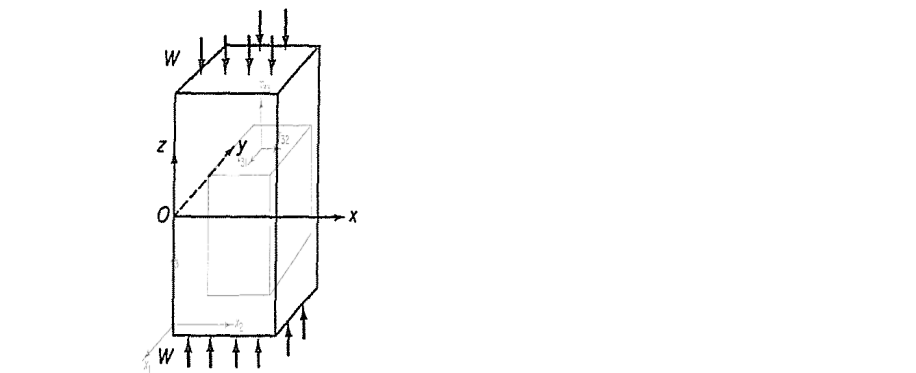
\includegraphics[width=.9\linewidth]{./images/FU94_1.11figure9a-uniaxial.png}
\end{center}
\end{itemize}
\begin{itemize}
\item Relabel coordinates (\(x\to x_1\), \(y\to x_2\), \(z\to x_3\)).
\item Take a section of the member using the  \(x_3\) plane from the \emph{mid-span} (region)

The mapping \(\boldsymbol{\nu} \to \boldsymbol{e}_3\) yields \(\overset{\nu}{\boldsymbol{t}} \to \overset{3}{\boldsymbol{t}}\)
\end{itemize}
\subsubsection*{Derivation of Nominal Normal Stress (Assumptions and Conventions)}
\label{sec:org948b05d}
About the traction flow, we assume that:
\begin{itemize}
\item there is no reason that the load \emph{would distribute non-uniformly} over the cross-section!! (i.e., there is \textbf{uniform distribution}, \(dW/dA = W/A\), leading to
$$ \overset{3}{t_3} = \tau_{33} = \sigma = \frac{W}{A}. $$
Here \(\sigma\) denotes the \textbf{nominal} \emph{normal} stress. It has units of load per area (e.g. N/cm\(^2\)).
\end{itemize}
\begin{itemize}
\item Under uniaxial loading, and in planes with normals parallel to the load axis, \textbf{only normal traction} arises (no shear tractions, i.e. \(\overset{3}{t_1} = \overset{3}{t_2} = 0\)).
\item Over planes that contain the load axis (whose normal will not not have an \(\boldsymbol{e}_3\) component), \textbf{zero traction} previals!! That means \(\overset{1}{\boldsymbol{t}}=\mathbf{0}\) and \(\overset{2}{\boldsymbol{t}}=\mathbf{0}\), which yield the state of stress
$$ [\tau] = \begin{bmatrix} 0 & 0 & 0 \\ 0 & 0 & 0 \\ 0 & 0 & \tau_{33} \end{bmatrix} $$
\item The given state of stress (having all shear terms identically zero) is also known as a state of \textbf{principal stress}.
\end{itemize}
\subsubsection*{Example: \href{https://openoregon.pressbooks.pub/bodyphysics2ed/chapter/stress-and-strain-on-the-body/}{Loading of the Femur}}
\label{sec:orgfa09e8c}
\url{./images/animation-femur.gif}

\begin{itemize}
\item Femur is the largest and most massive bone in the our body.
\begin{enumerate}
\item Assume the load component in the axial-plane to be negligible?? (which is the same as saying the load is entirely axial and no shear component is taken)
\item Using average values for a standard female, determine the normal compressive stress. (search keywords: CDC standard anthropometric measurements female data)
\item Knowing the femur axis deviates from the vertical (gravity axis) on the average by some small angle (e.g. 9 degrees), what is a more realistic state of stress?
\end{enumerate}
\end{itemize}

State of Stress on a Plane that is Not Normal to the Load.
\begin{center}
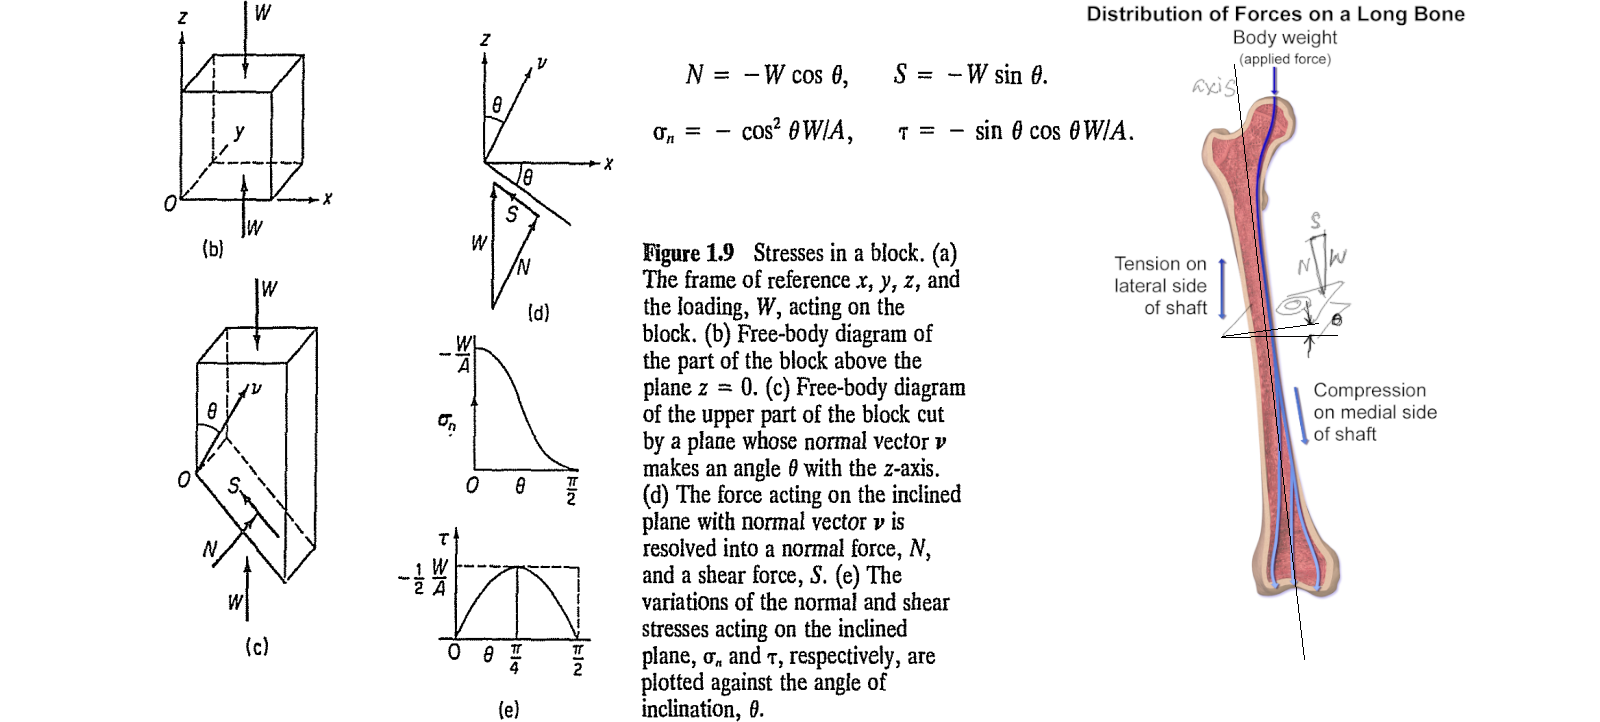
\includegraphics[width=.9\linewidth]{./images/FU94_1.11figure9c-mod.png}
\end{center}
\begin{itemize}
\item Assume a deviation of 8 degrees between the axial load and the femoral axis, determine the shear stress to normal stress ratio observed on an axial plane.
\end{itemize}
\subsection*{Plates under Plane Stress}
\label{sec:orgd567a02}
\subsubsection*{Plane State of Stress}
\label{sec:orgbca9b12}
\begin{itemize}
\item thin flat plates or membranes stretched by in-plane load systems
\begin{center}
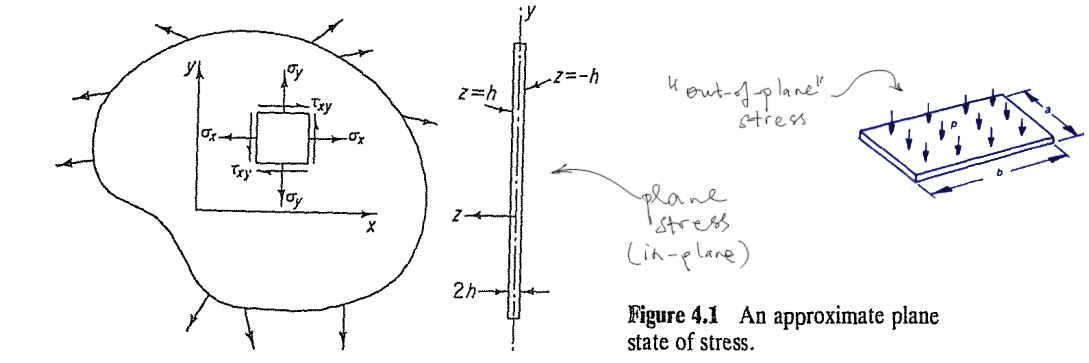
\includegraphics[width=.9\linewidth]{./images/FU94-fig4.1.png}
\end{center}
\end{itemize}
\begin{itemize}
\item found in ship hulls, pressurized bodies, wings, panels
\item under these conditions the \emph{out-of-plane} stress components vanish.
\item if you choose a reference coordinate frame whose any two axes lie along the plate's plane, then you get a reduced stress tensor, such that (continue to next section)
\end{itemize}
\subsubsection*{Reduction of the Stress Tensor to 2-D}
\label{sec:orgd00f17b}
\begin{itemize}
\item We may choose the plate coordinate pair to be \((1,2)\), \((2,3)\), or \((1,3)\), in which cases the corresponding stress tensors would read:
$$ \tau_{ij} = [\tau] = \begin{bmatrix}  \tau_{11} & \tau_{12} & 0 \\ \tau_{21} & \tau_{22} & 0 \\ 0 & 0 & 0 \end{bmatrix}, \, \{i,j=1,2\}, \quad \begin{bmatrix} 0 & 0 & 0 \\ 0 & \tau_{22} & \tau_{23} \\ 0 & \tau_{32} & \tau_{33} \end{bmatrix}, \, \{i,j=2,3\}, \quad  \mathrm{or}, \; \begin{bmatrix}  \tau_{11} & 0 & \tau_{13} \\ 0 & 0 & 0 \\ \tau_{31} & 0 & \tau_{33} \end{bmatrix}, \, \{i,j=1,3\} $$
\end{itemize}
\begin{itemize}
\item The two non-zero coordinate components can be combined in a \emph{reduced} stress tensor, depicting the \emph{state of plane stress} as
$$ \tau_{ij} = [\tau] = \begin{bmatrix}  \tau_{11} & \tau_{12} \\ \tau_{21} & \tau_{22} \end{bmatrix}, \, \{i,j=1,2\} $$
\item There is no special symbol or indicator, whatsoever, that is used when the dimension of space is reduced from 3 to 2, \([\tau]\) prevails. The dimensionality is understood from the context.
\end{itemize}
\subsubsection*{The Scapula (A flat bone)}
\label{sec:org6ca3605}
\begin{center}
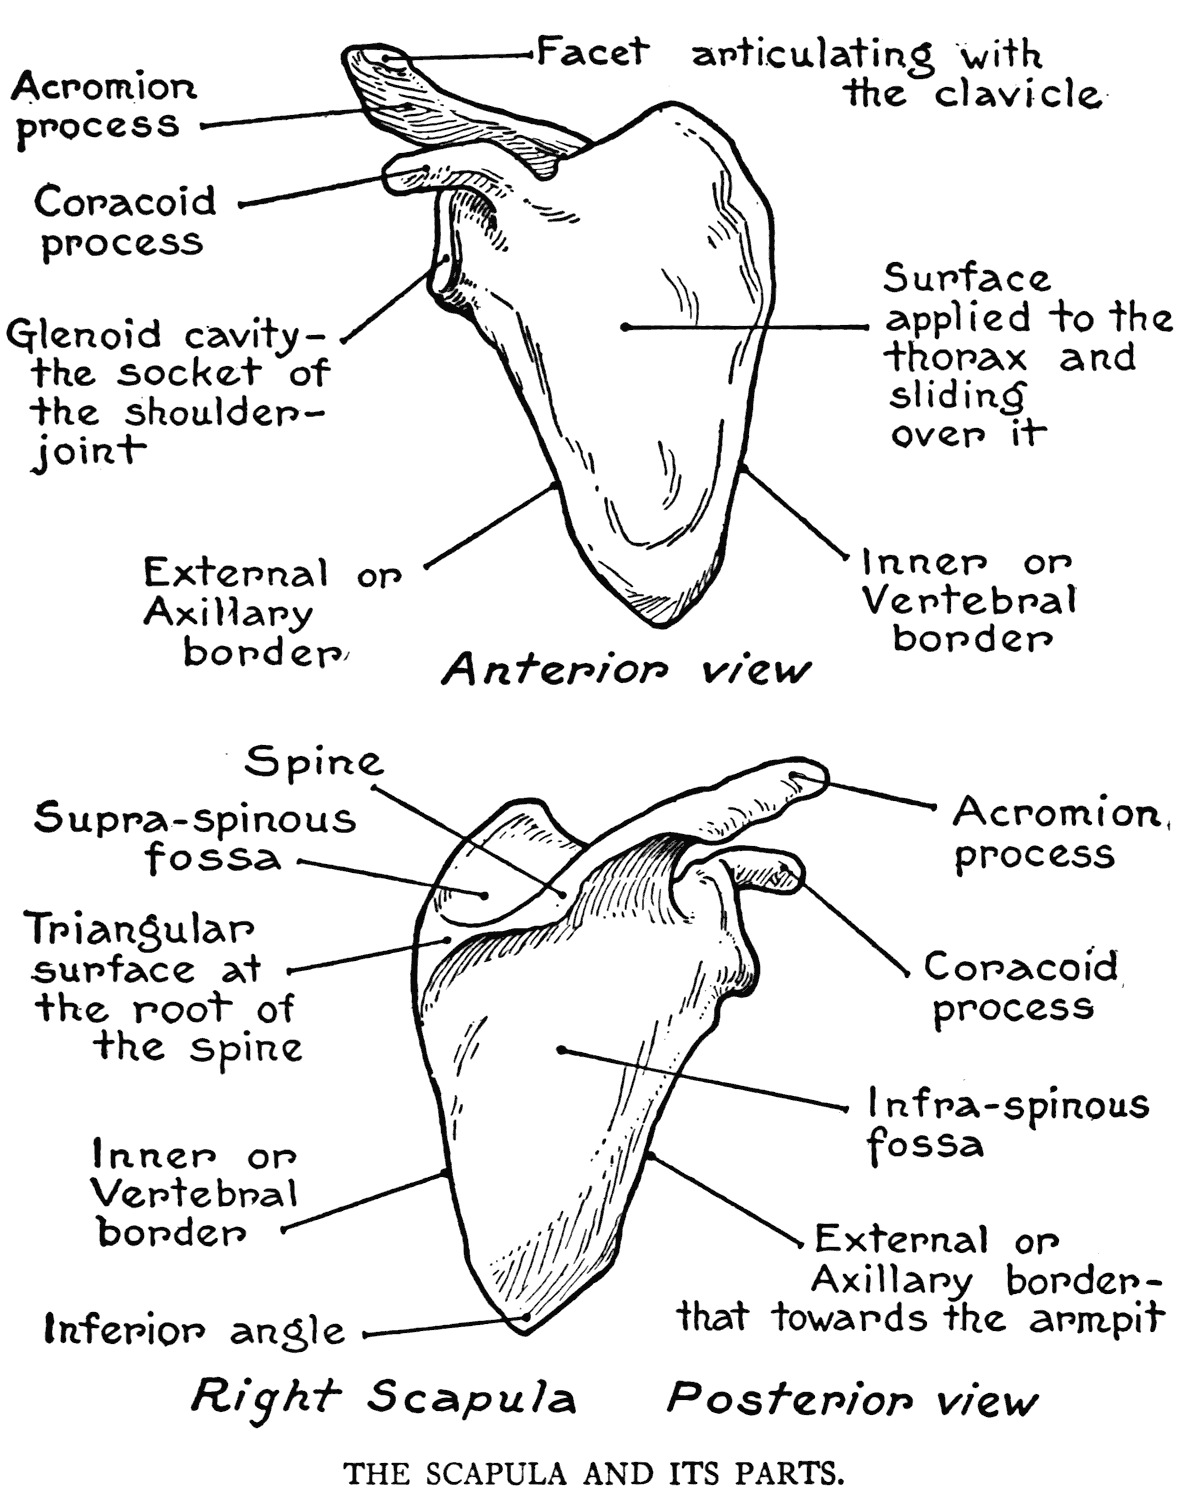
\includegraphics[width=.9\linewidth]{./images/fig1.11.4scapula.jpg}
\end{center}
\subsubsection*{Loading and Fracture of Scapula}
\label{sec:orgee74891}
\begin{itemize}
\item The state of \emph{in-plane loading} of the scapula, and the most frequently observed \textbf{fracture modes} (according to \href{https://orthoinfo.aaos.org/en/diseases--conditions/scapula-shoulder-blade-fractures/}{OrthoInfo})
\begin{center}
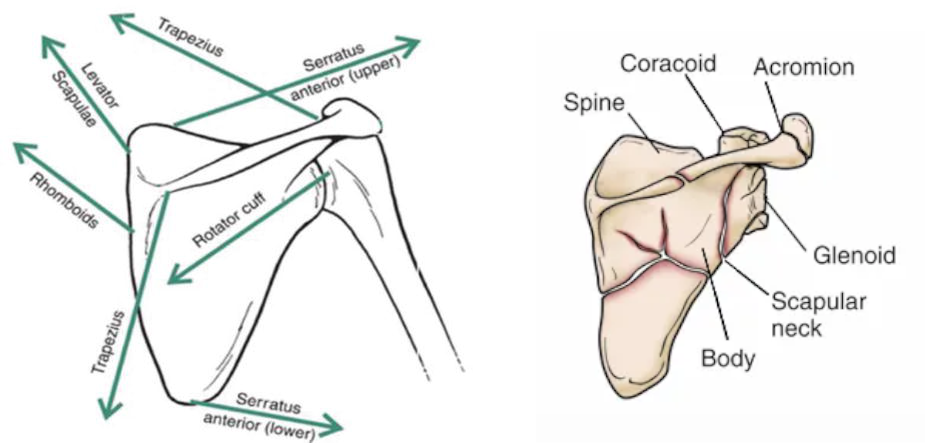
\includegraphics[width=.9\linewidth]{./images/fig1.11.4scapulaFBD.png}
\end{center}
\end{itemize}
\begin{itemize}
\item A nominal stress calculation does not exist for this case (details about loading and boundary restraints should be provided to pose a proper \emph{boundary-value problem})
\end{itemize}
\subsection*{Stresses in Pressurized Vessels}
\label{sec:org472763a}
Many biological examples of pressurized biological tissue may be provided.
\begin{itemize}
\item Lung tissue: Maintains subatmospheric interstitial pressure (−2 to −9 mmHg) due to elastic recoil, crucial for alveolar expansion and gas exchange.
\item Kidney: Encapsulated organ with positive interstitial pressure (up to +10 mmHg), aiding fluid filtration and urine formation.
\item Vasculatory system components, veins are pressurized biological tissues, but they operate under much lower pressure compared to arteries.
\end{itemize}
\section*{(\(\S3.2\)) Laws of Motion}
\label{sec:org6dc4806}
\begin{itemize}
\item Let the space occupied by a material body \(B\) at time \(t\), be denoted it's configuration \(B(t)\).
\item Let \(\boldsymbol{r}\) denote the position vector of a material point \(X\).
\item Utilize cartesian coordinates \(x_i,\,i=1,2,3\) for spatial meaurements.
\item Consider a differential volume element \(dv\) around \(X\).
\item Let \(\rho\) denote the mass density field and \(\boldsymbol{v}=\dot{\boldsymbol{r}}\) denote the velocity field in \(B\).
\end{itemize}
\subsection*{Balance of Mass}
\label{sec:orgbee2999}
\begin{itemize}
\item The total mass of the material configuration \(B(t)\) can be expressed by integration.
\item We can denote the mass enclosed in \(dV\) by \(\rho dV\).
\item Then the total mass of \(B\) at time \(t\) becomes
$$ \mathcal{M} = \int_{B(t)} \rho dV $$
\item The rate of change of the total mass is shown by
$$ \dot{\mathcal{M}} = \frac{D \mathcal{M}}{Dt} = \frac{D}{Dt} \int_{B(t)} \rho dV = \int_{B(t)} \frac{D}{Dt} (\rho dV) = \int_{B(t)} (\rho dV)^{\!\bullet}  $$
where \(\frac{D}{Dt}(\ldots)\) and \((\ldots)^{\!\bullet}\) denote the \emph{material time derivative} operator, taking the derivative with respect to configurational changes of the material body \(B\) with time.
\item The conservation of mass of a body is expressed by setting
$$ \dot{\mathcal{M}} = 0 $$
\end{itemize}
\begin{itemize}
\item Notes of Importance
\label{sec:orgba37eda}
\begin{enumerate}
\item the balance of mass states that the net change in mass is given by the material time rate of the mass integral, \(\dot{\mathcal{M}}\).
\item the role of material time derivative to highlight the difference between \(\int_B (\cdots)^{\!\bullet}\) and \(\int_{B(t)} (\cdots)^{\!\bullet}\)
\item Ask GPT:
\begin{quote}
How would you describe the difference between a time derivative in the usual (\emph{partial}) sense and that for a body in motion in the \textbf{total} sense? If possible, supply an image of a traveling (material) window versus a fixed (spatial) window highlighting the difference between tracking the motion of a group of particles versus observing the flow through a control volume.
\end{quote}
\end{enumerate}
\end{itemize}
\subsection*{Balance of Linear Momentum}
\label{sec:org77299ed}
\begin{itemize}
\item The total linear momentum of the material configuration \(B(t)\) can also be expressed by integration.
\item We denote the linear momentum of the mass \(\rho dV\) by multiplying it with its velocity as \(\boldsymbol{v} \rho dV\).
\item Then the total linear momentum of \(B\) at time \(t\) becomes
$$ \mathcal{P} = \int_{B(t)} \boldsymbol{v} \rho dV $$
\item Euler interpreted Newton's equation of motion of a particle for a body by stating that the rate of change of linear momentum is equal to the resultant of all external mechanical effects (loads) as
$$ \dot{\mathcal{P}} = \mathcal{F} $$
where \(\dot{\mathcal{P}}\) denotes the material time derivative of the linear momentum and \(\mathcal{F}\) denotes the net external force on \(B\).
\end{itemize}
\subsubsection*{Classification of External Loads}
\label{sec:org20dd191}
\begin{itemize}
\item In the mechanics of continuous media, there are two types of external forces acting on material bodies.
\begin{enumerate}
\item Body forces, acting on volume elements (forces per unit volume).
\begin{itemize}
\item \(\boldsymbol{X}\) or \(\boldsymbol{b}\)
\item gravitational loads (\(\rho \boldsymbol{g}\) has units of force per volume)
$$ \int_{B(t)} \boldsymbol{b} dV = \int_{B(t)} \boldsymbol{g} \rho dV$$
\item electromagnetic loads
\end{itemize}
\item Surface forces, or surface tractions, acting on surface elements (forces per unit area).
\begin{itemize}
\item surface traction due to mechanical contact
$$ \overset{\nu}{\boldsymbol{T}} \quad \mathbf{or} \quad \overset{\nu}{\boldsymbol{t}} \quad \to \quad \int_{\partial B(t)} \overset{\nu}{\boldsymbol{t}} dA $$
\item aerodynamic pressure (units of force per area), \(-p\boldsymbol{n}\)
where \(\boldsymbol{n}\) is the unit outward normal at the surface of \(B\).
\item drag force in viscous flows
\end{itemize}
\end{enumerate}
\end{itemize}
\subsubsection*{Balance of Linear Momentum (with forces)}
\label{sec:org0e57b0f}
Replacing the general expression of the resultant of external forces, \(\mathcal{F}\) with the above force type definitions, we arrive at the terminal integral expression
$$ \int_{\partial B(t)} \overset{\nu}{\boldsymbol{t}} dA +  \int_{B(t)} \boldsymbol{b} dV =  \int_{B(t)} (\boldsymbol{v} \rho dV)^{\!\bullet} $$
\subsection*{Balance of Moment of Momentum}
\label{sec:orgad50fcc}
\begin{itemize}
\item The integral of the moment of momentum of the differential mass element about the origin \(O\), \(\boldsymbol{r} \times \boldsymbol{v} \rho dV\), over the domain \(B(t)\), i.e.,
$$ \mathcal{H}^O = \int_{B(t)} \boldsymbol{r} \times \boldsymbol{v} \rho dV $$
is the \emph{moment of momentum} of the configuration at \(B(t)\).
\item According to Euler, the law of motion for a continuum asserts that the \emph{rate of change of the moment of momentum is equal to the net applied torque \(\boldsymbol{r} \times \mathcal{F}\) about the origin}, i.e.,
$$ \dot{\mathcal{H}}^O = \boldsymbol{r} \times \mathcal{F} $$
\item Replacing \(\mathcal{F}\) with the force definitions, we the second vector equation of motion
$$ \int_{\partial B(t)} \boldsymbol{r} \times \overset{\nu}{\boldsymbol{t}} dA +  \int_{B(t)} \boldsymbol{r} \times \boldsymbol{b} dV =  \int_{B(t)} (\boldsymbol{r} \times \boldsymbol{v} \rho dV)^{\!\bullet} $$
\end{itemize}
\section*{(\(\S3.3\)) Cauchy's Formula}
\label{sec:org09736e0}
Relates the components of the traction that resides over a plane with a normal \(\nu\), with the unit normal and the stress tensor components.
$$ \overset{\nu}{t_j} = \nu_i \tau_{ij} $$
Note that similar relations between the traction vector components on cartesian planes, the base vector and stress tensor components exists:
\begin{align}
 \overset{1}{t_j} & = \boldsymbol{e}_{1i} \tau_{ij} \\
 \overset{2}{t_j} & = \boldsymbol{e}_{2i} \tau_{ij} \\
 \overset{3}{t_j} & = \boldsymbol{e}_{3i} \tau_{ij} \\
\end{align}

\begin{center}
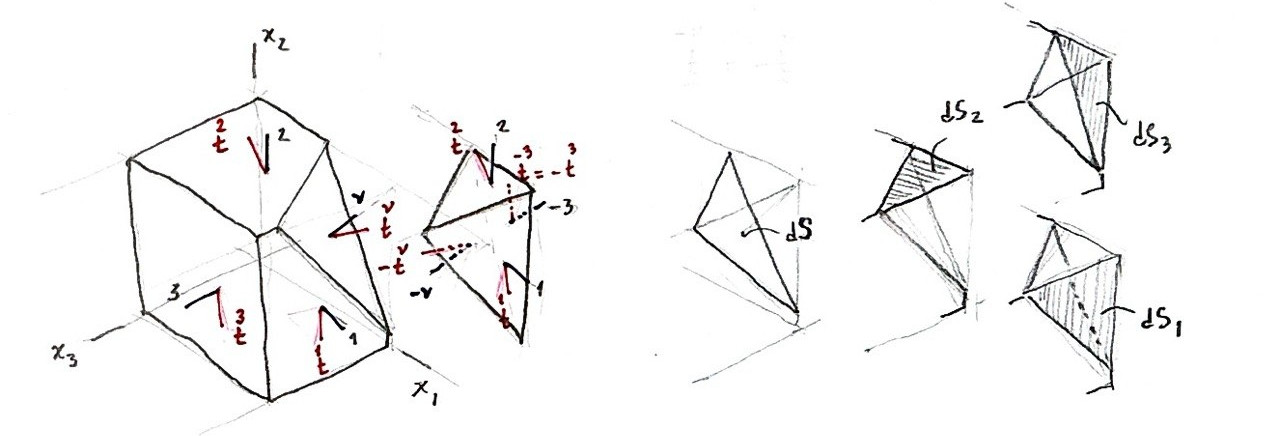
\includegraphics[width=.9\linewidth]{./images/fig3.3-cubecut.jpg}
\end{center}
\begin{itemize}
\item The internal surface traction at a point \(P\) over a plane with a normal \(\nu\) was defined by \(\overset{\nu}{\boldsymbol{T}}\) or \(\overset{\nu}{\boldsymbol{t}}\). The traction over the opposite plane (with a normal \(-\nu\)) is equal in magnitude but opposite in direction, i.e. \(\overset{-\nu}{\boldsymbol{t}} = -\overset{\nu}{\boldsymbol{t}}\).
\item This is also true for the tractions that lie over cartesian planes, e.g.  \(\overset{-1}{\boldsymbol{t}} = -\overset{1}{\boldsymbol{t}}\), etc.
\item From geometry, we define the area formed by the intersection of an oblique plane with normal \(\nu\), and the three other cartesian planes, as \(dS\).
\item The projection of \(dS\) onto the cartesian plane \(i\) (perpendicular to \(x_i\)) is given by \(dS_i = \nu_i dS\).
\end{itemize}
\subsection*{Motion Law Applied to a Tetrahedron Cut}
\label{sec:org08c48e2}
\begin{center}
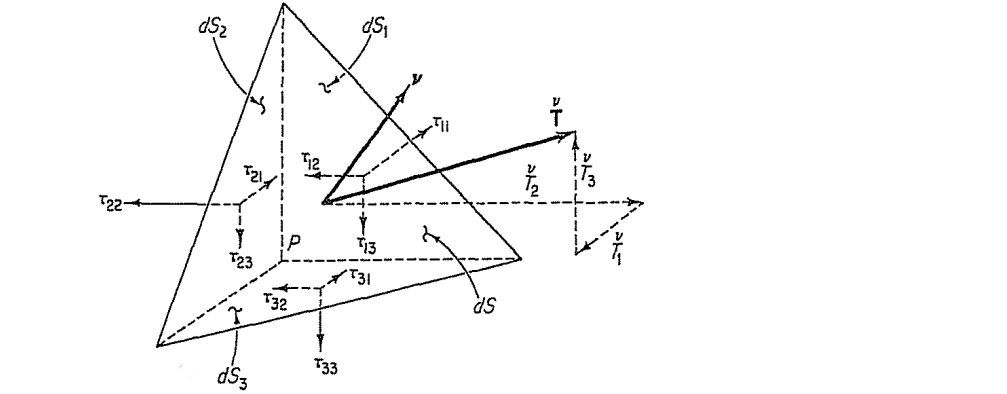
\includegraphics[width=.9\linewidth]{./images/FU94_3.3figure5.png}
\end{center}
\begin{itemize}
\item For the tetrahedron cut with four surfaces (\(dS_i, dS\)) and volume \(dV={{1}\over{3}}h dS\):
\item Surface forces: \(-\overset{1}{\boldsymbol{t}} dS_1\), \(-\overset{2}{\boldsymbol{t}} dS_2\), \(-\overset{3}{\boldsymbol{t}} dS_3\) on cartesian planes and \(\overset{\nu}{\boldsymbol{t}} dS\) on the oblique plane
\item Body force: \(\boldsymbol{b} {{1}\over{3}}h dS\).
\item Inertial term: \(\dot{\boldsymbol{v}} {{1}\over{3}}h dS\).
\end{itemize}

\begin{center}
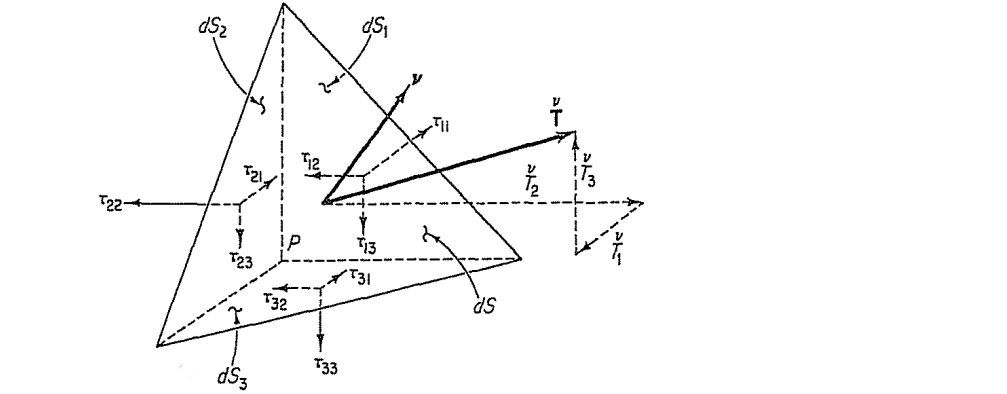
\includegraphics[width=.9\linewidth]{./images/FU94_3.3figure5.png}
\end{center}
\begin{itemize}
\item The balance of linear momentum for the tetrahedron cut reads:
$$ -\overset{1}{\boldsymbol{t}} dS_1 - \overset{2}{\boldsymbol{t}} dS_2 - \overset{3}{\boldsymbol{t}} dS_3 + \overset{\nu}{\boldsymbol{t}} dS + \boldsymbol{b} {{h}\over{3}} dS = \dot{\boldsymbol{v}} {{h}\over{3}} dS $$
\end{itemize}
\begin{itemize}
\item Replacing \(dS_i = \nu_i dS\), dividing by \(dS\), and taking the limit as \(h \to 0\), we obtain
$$ \overset{\nu}{\boldsymbol{t}} = \nu_1 \overset{1}{\boldsymbol{t}} + \nu_2 \overset{2}{\boldsymbol{t}} + \nu_3 \overset{3}{\boldsymbol{t}} $$
\end{itemize}

\begin{center}
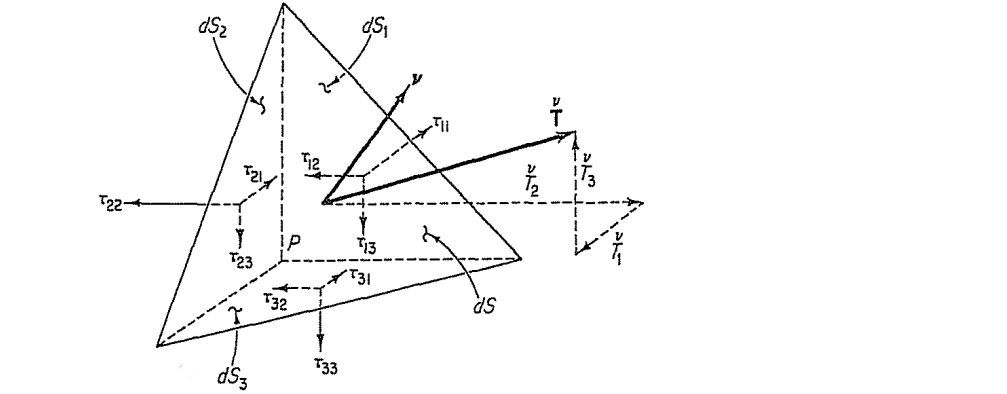
\includegraphics[width=.9\linewidth]{./images/FU94_3.3figure5.png}
\end{center}
\begin{itemize}
\item Arranging the components \(\nu_i\) in a vector form and the vectors \(\overset{i}{\boldsymbol{t}}\) in a matrix form yields
$$ \overset{\nu}{\boldsymbol{t}} = \{\nu_1\; \nu_2\; \nu_3 \} \begin{bmatrix} -\; \overset{1}{\boldsymbol{t}} \to \\ -\; \overset{2}{\boldsymbol{t}} \to \\ -\; \overset{3}{\boldsymbol{t}} \to \end{bmatrix} $$
\end{itemize}
\begin{itemize}
\item and noting that the matrix components \(\overset{i}{t}_j\) corresponds identically with the stress tensor components \(\tau_{ij}\), we get the Cauchy's Formula \(\overset{\nu}{t}_j = \nu_i \tau_{ij}\).
\end{itemize}
\subsubsection*{Sample Problem 1: (\href{./Ch2-vectors.html}{use plane formula})}
\label{sec:org9c429e1}
\begin{center}
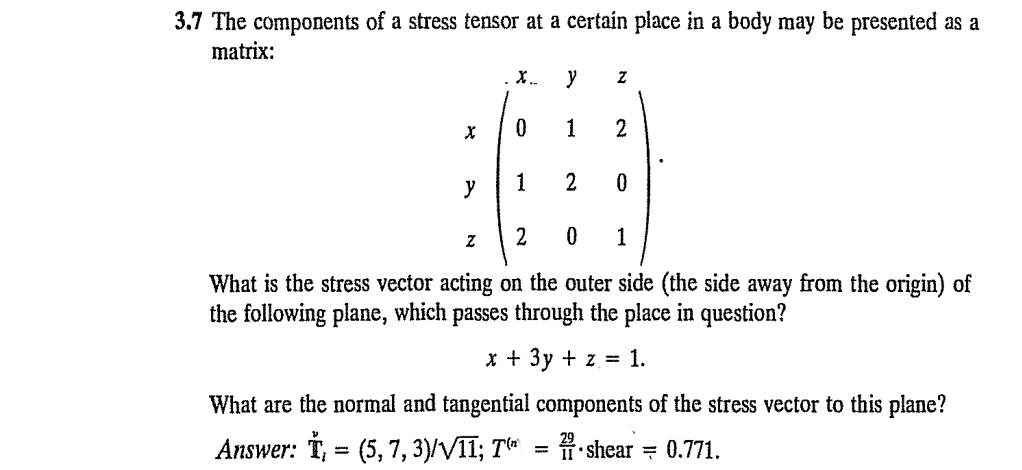
\includegraphics[width=.9\linewidth]{./images/FU94_3.3problem7.png}
\end{center}
\subsubsection*{Sample Problem 2}
\label{sec:org6b291d2}
\begin{center}
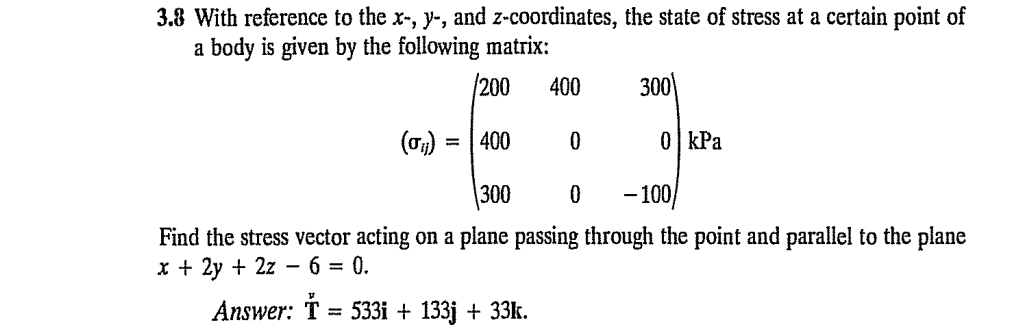
\includegraphics[width=.9\linewidth]{./images/FU94_3.3problem8.png}
\end{center}
\section*{(\(\S3.5\)) Transformation of Stress Components}
\label{sec:orgca18b28}
Remember how coordinates of a point, \(x_j\), could be transformed from the basis \(\boldsymbol{e}_j\) into another bases \(\boldsymbol{e}_{i'}\)?
\begin{itemize}
\item We used the rotation tensor definition \(\beta_{i'j} = \boldsymbol{e}_{i'} \cdot \boldsymbol{e}_j\) for this purpose, and wrote the transformed coordinates as
$$ x_{i'} = \beta_{i'j} x_j $$
\item Can this approach be used to transform the stress tensor components, \(\tau_{ij} \to \tau_{i'j'}\)?
\end{itemize}
\subsection*{The Rotation Tensor Transforms a Second-Order Tensor}
\label{sec:org6309b9a}
\begin{center}
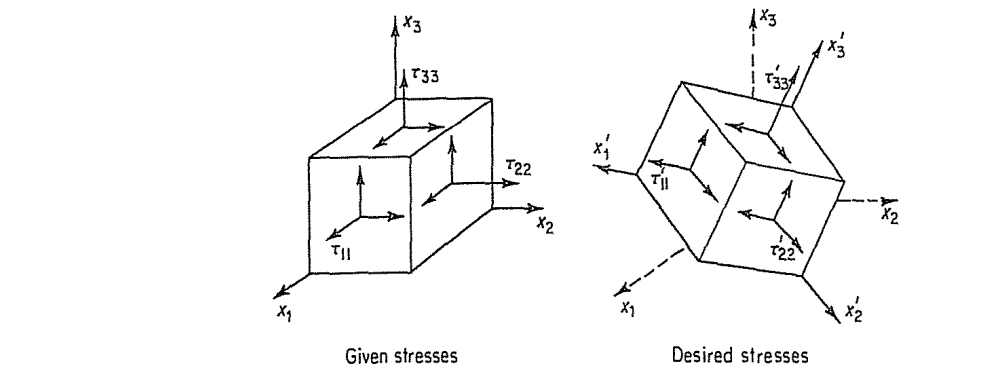
\includegraphics[width=.9\linewidth]{./images/FU94_3.5figure9.png}
\end{center}
\begin{itemize}
\item Stress is a second-order tensor with two indices \(\tau_{ij}\) where the components are expressed with respect to a particular coordinate frame using a set of basis vectors, \(\boldsymbol{e}_i\).
\item Consider an alternative coordinate frame using it's own set of basis vectors, \(\boldsymbol{e}_{j'}\).
\item How are the stress components in the two frames, \(\tau_{ij}\) and \(\tau_{i'j'}\) related?
\end{itemize}

\begin{center}
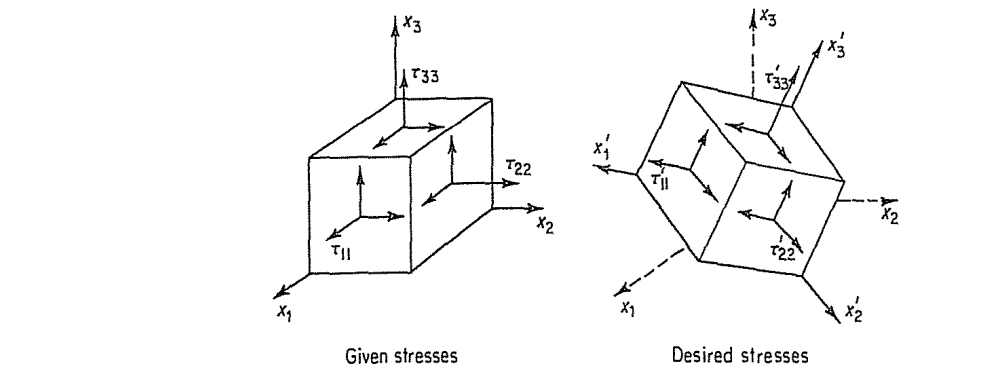
\includegraphics[width=.9\linewidth]{./images/FU94_3.5figure9.png}
\end{center}
\begin{itemize}
\item As it turns out each one of the indices of a higher-order tensor can be and should be transformed by a coordinate transformation operation
\end{itemize}
\begin{itemize}
\item Thus, for a second-order tensor such as stress, two transformations are in order, as
$$ \tau_{i'j'} = \beta_{i'i} \beta_{j'j} \tau_{ij}. $$
\item Noting the order in which inner product takes place, the matrix form reveals
$$ [\tau'] = [\beta] [\tau] [\beta]^T $$
where a normal matrix multiplication occurs in a row-column operation which a transposed multiplication occurs in a column-column operation.
\end{itemize}
\subsubsection*{Educational Application Hub:}
\label{sec:org2165f99}
Tools for transforming components of the second-order stress tensor
\begin{itemize}
\item \url{https://eduapphub.com/apps/app.php?dir=2Dstresstransform}
\item \url{https://eduapphub.com/apps/app.php?dir=3Dstresstransform}
\end{itemize}
\subsubsection*{Sample Problem 1}
\label{sec:org68e74ca}
\begin{center}
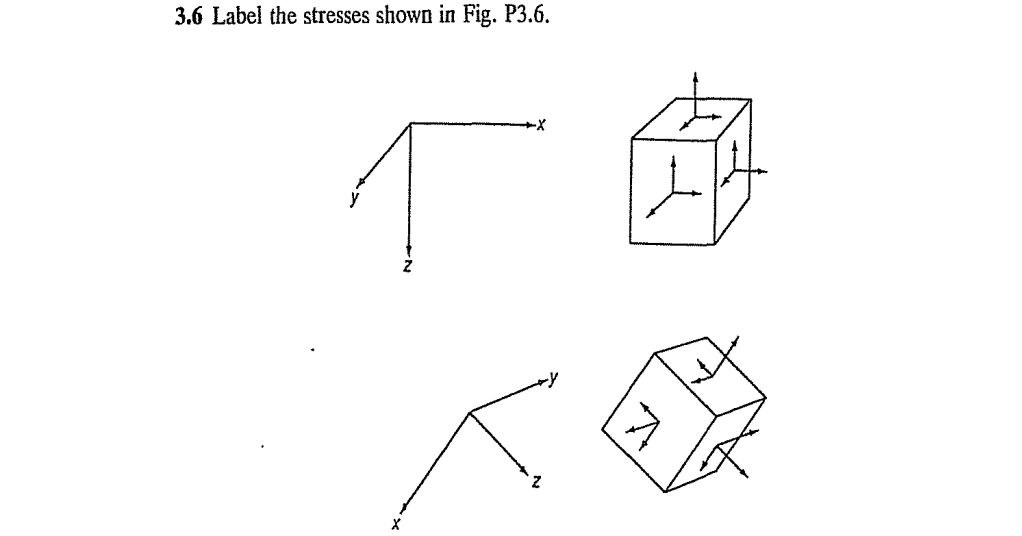
\includegraphics[width=.9\linewidth]{./images/FU94_3.4problem6.png}
\end{center}
\subsubsection*{Sample Problem 2}
\label{sec:org6123956}
\begin{center}
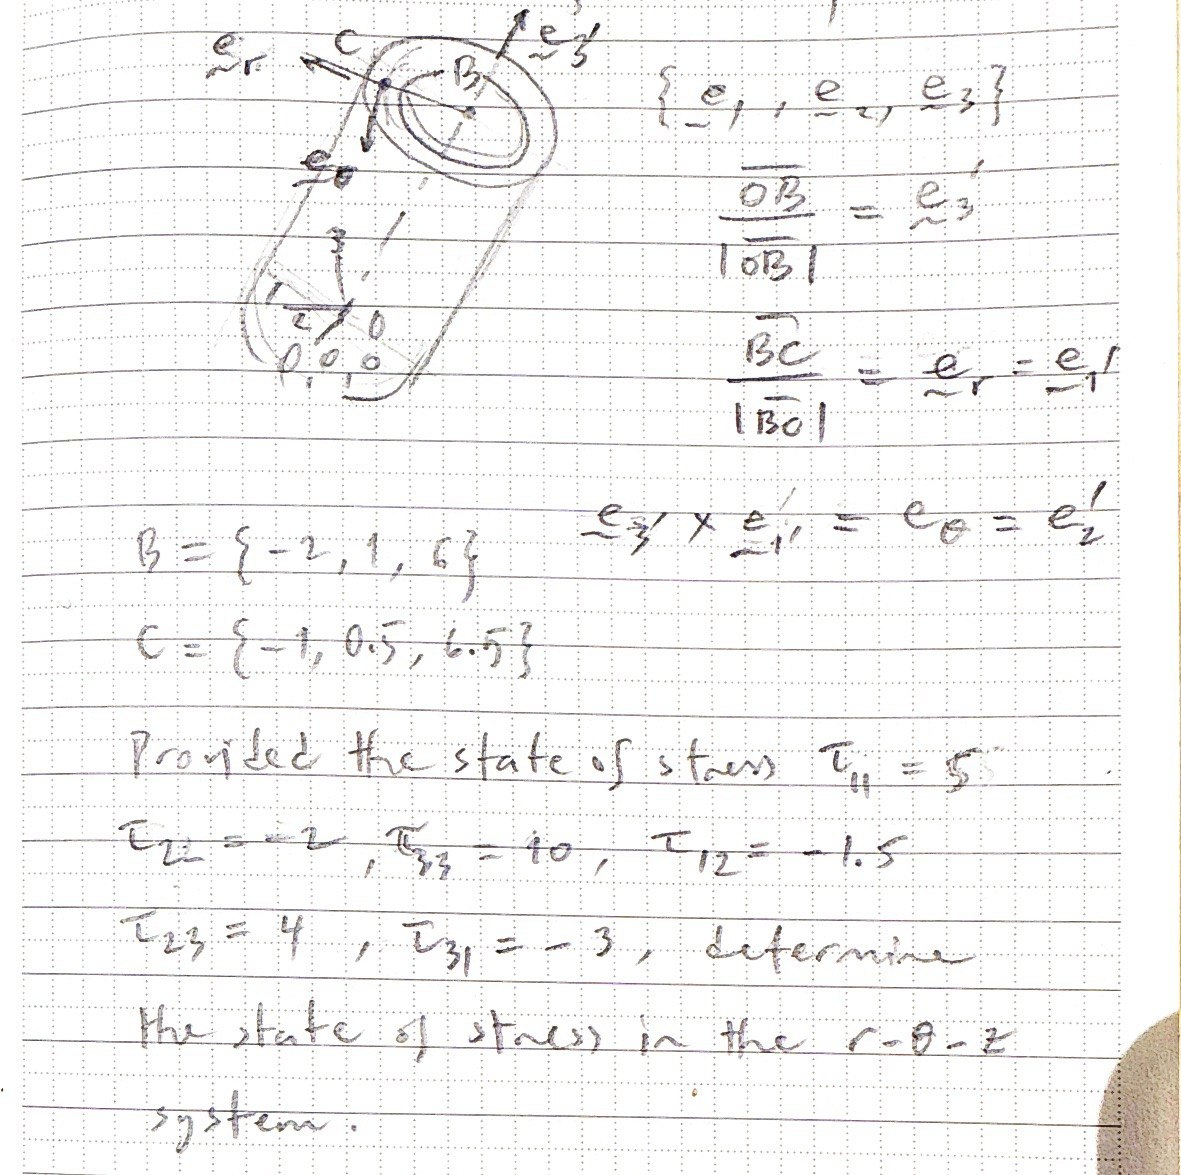
\includegraphics[width=.9\linewidth]{./images/fig3.4-problem1.jpg}
\end{center}

\begin{itemize}
\item Initial script produced in class
\begin{verbatim}
B = [-2 1 6]  % point definition, upper end of axis
C = [-1 0.5 6.5] % point definition, state of stress is given here
BC = C - B   % line segment from axis (is this perpendicular to OB?)
e_1p = BC / norm(BC)   % e_r ?? 
e_3p = [0 0 1]         % e_z ??
e_2p = cross(e_3p,e_1p)
beta=[e_1p;e_2p;e_3p]
\end{verbatim}
\item Two problems with this script can be identified
\begin{enumerate}
\item the cylinder axis may not be aligned with \(x_3\)
\item Segment BC may not be purely radial
\end{enumerate}
\item Corrected script     
\begin{verbatim}
e_BC = BC / norm(BC)   % vector may not be radial, do not call it e_1p
e_3p = B / norm(B)     % vector e_3p is not [0 0 1], OB -> B
C_3p = dot(C,e_3p)     % scalar projection of C onto e_3p
CT3p = C - C_3p*e_3p   % vector component of C perpendicular to e_3p
e_1p = CT3p / norm(CT3p)  
e_2p = cross(e_3p,e_1p)
beta=[e_1p;e_2p;e_3p]
\end{verbatim}
\end{itemize}
\section*{(\(\S3.7\)) Boundary Conditions}
\label{sec:orgfc3a8f6}
Describing various state of stress conditions that arise in bodies.
\begin{itemize}
\item condition of a body submerged in a fluid
\begin{itemize}
\item a building subjected to wind
\item a vessel wall subjected to internal pressure
\end{itemize}
\item condition at a bimaterial interface
\begin{itemize}
\item relative sliding and contact between bodies
\item sticking interface (various joining methods exist)
\end{itemize}
\item condition of point loads (singularities)
\begin{itemize}
\item point forces and force couples
\end{itemize}
\end{itemize}
We know something about the forces or motion on the surface of a solid or a fluid and inquire what happens within \ldots{}
\subsubsection*{A Bimaterial Square Block Under Axial Contraction}
\label{sec:orgc3ff9a2}
\begin{center}
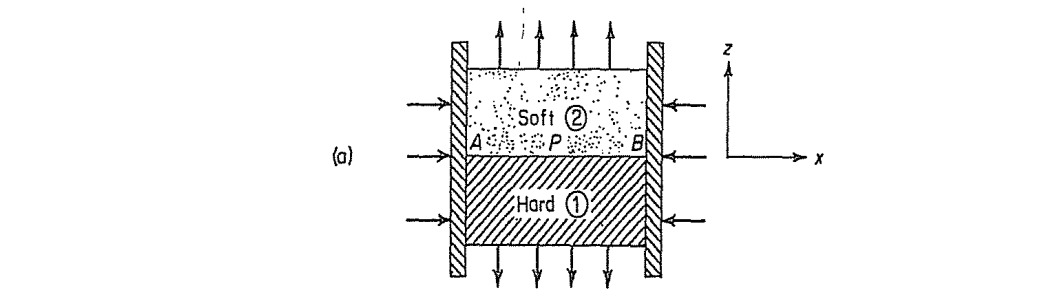
\includegraphics[width=.9\linewidth]{./images/FU94_3.7figure11a.png}
\end{center}
\begin{itemize}
\item Imagine the square is made of a soft upper half and a hard lower part joined together by the middle horizontal line.
\end{itemize}
\begin{itemize}
\item Let the square block be compressed by the lateral side walls on the left and right. What will be the state of stress at the bimaterial interface?
\item How will the state of stress change within each body?
\end{itemize}

\begin{center}
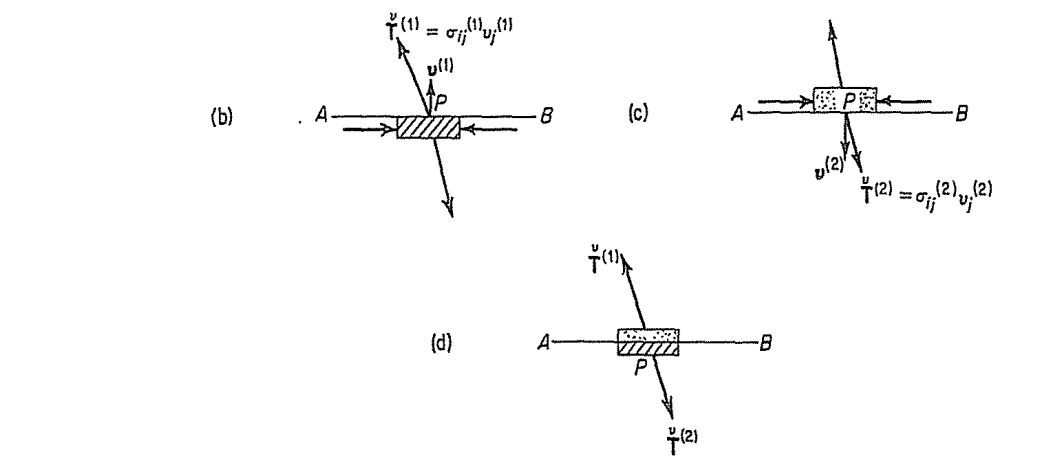
\includegraphics[width=.9\linewidth]{./images/FU94_3.7figure11bcd.png}
\end{center}
\begin{itemize}
\item From the interface, traction vector changes slightly within the soft part (a), and the hard part (b)
\end{itemize}
\begin{itemize}
\item At the interface, boundary condition requires the \emph{continuity of traction}, i.e. \(\overset{i}{t}^{(1)} = \overset{i}{t}^{(2)}\).
\end{itemize}
\subsubsection*{What is external?}
\label{sec:org1cdd9cb}
\begin{center}
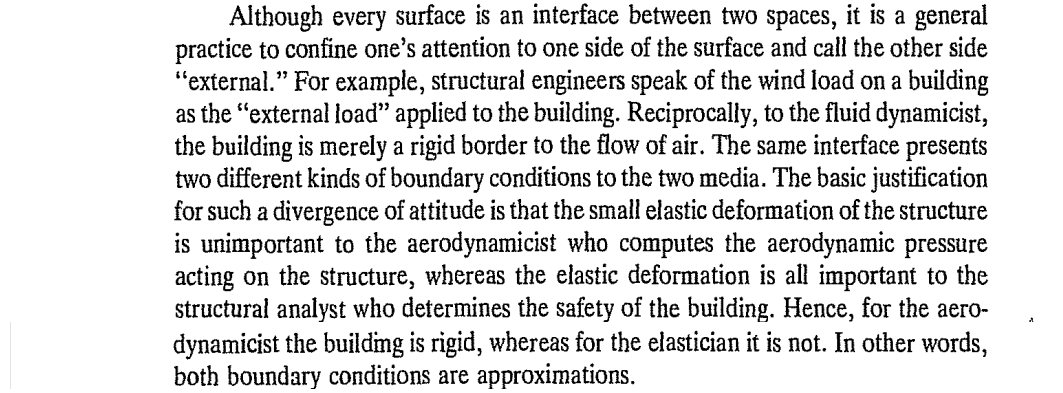
\includegraphics[width=.9\linewidth]{./images/FU94_3.7paragraph.png}
\end{center}
\subsection*{Sample Problem: Hydrostatic Stress}
\label{sec:org0f8253b}
\begin{center}
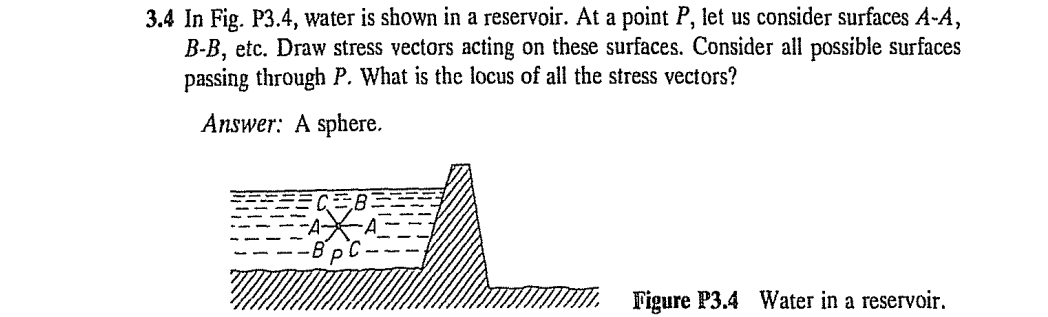
\includegraphics[width=.9\linewidth]{./images/FU94_3.7problem4.png}
\end{center}
\end{document}
